%%%% Ecriture du plan

Au commencement était l'information. Et l'information était à gérer, et l'information posa problème. Les développeurs de logiciels qui travaillaient en équipe devaient se soucier de mettre en commun leurs modifications. 
Nous étions à la préhistoire de l'informatique.
% (ère qui n'est peut-être pas révolue de nos jours, comme nous verrons par la suite)

\section{Problématiques et historique}

\subsection{Mauvaises pratiques}



Plusieurs solutions furent envisagées, des plus téméraires aux plus banales:
\begin{itemize}
\item CPOLD : pour mettre en commun une modification, nous gardions une copie du fichier d'origine, renommé en \texttt{.old} et nous copions le nouveau fichier sur un répertoire commun. Ceci est issu d'un article fake du net ~\cite{CPOLD-article}. 
\item La solution de la disquette : chaque modification pouvait être transmise par un nouveau fichier via une disquette, un e-mail ou autre.
\item De nos jours encore, certaines personnes utilisent un service de synchronisation dans le cloud (du type Dropbox/SugarSync) pour synchroniser leurs fichiers et dossiers sur tous les ordinateurs. 
\end{itemize}

Ces façons de gérer les ressources présentaient de nombreux défauts. Nous pouvons noter en particulier : 
\begin{enumerate}
\item le manque de robustesse et la perte de données possibles en cas d'erreur lors de la copie ;
\item l'impossibilité de remonter aux anciennes versions des fichiers ;
\item la redondance de l'information. Une grande partie des modifications n'affecte pas l'ensemble du fichier ;
\item le manque d'automatisation. Les opérations étaient réalisées à la main -- ou au mieux à l'aide de scripts bash, MDR! 
\end{enumerate}

\subsection{L'invention du gestionnaire de versions}

Nous sommes dans les années 80, l'essor du logiciel libre attire de plus en plus de développeurs. 
Ceux-ci collaborent sur des projets dont la complexité s'accroît au cours du temps. 
La gestion de projets d'une telle envergure nécessite des outils adaptés. 
Afin de répondre aux problématiques sus-citées, ils ont développé plusieurs solutions. 

\subsection{Généalogie}

Puis ils se marièrent et eurent beaucoup d'enfants. L'arbre donné en figure \ref{fig:chronologie} retrace leur généalogie. 


\begin{figure}[h!]
  \centerline{
  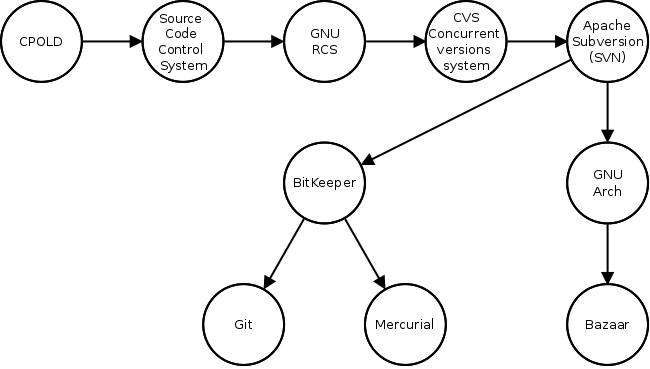
\includegraphics[width=14cm]{images/chronologie.png}}
  \caption{Résumé des gestionnaires de versions à travers l'histoire}
  \label{fig:chronologie}
\end{figure}

RCS engendra CVS. CVS engendra SVN. SVN fut fécond et insuffla la vie à deux enfants, BitKeeper et GNU Arch. 
Puis BitKeeper, qui était un projet propriétaire voulut devenir open source. De cette séparation naquirent Mercurial et GIT. 

Ce qui suit est tiré d'un article du net \cite{Article-hist-A}. 

\subsubsection{RCS (Revision Control System)}

La première solution stable sortit dans le cadre du projet GNU, initié par Richard Stallman. Il s'agit de RCS (acronyme pour Revision Control System) ~\cite{GNUWebSite}. 
Celui-ci est une amélioration de SCCS (Source Code Control System). Il présente une interface plus simple d'utilisation, un stockage amélioré des versions de fichiers afin de les retrouver plus rapidement. 

\subsubsection{CVS (Concurrent Versions System)}

Le concept était important, mais encore inadapté dans le cadre d'un projet logiciel impliquant un arbre de fichiers et toute une équipe projet. C'est pourquoi, au début des années 1990 s'est développé le célèbre CVS, logiciel destiné à permettre à des équipes de développer des projets complets. Techniquement, CVS s'appuie sur son prédécesseur RCS, en lui ajoutant une couche de transmission de fichiers par le réseau, et une autre de gestion de plusieurs fichiers (toutefois indépendants les uns des autres). Voici ce que dit l'auteur original des premières lignes de CVS :

\begin{quotation}
I created CVS to be able to cooperate with my students, Erik Baalbergen and Maarten Waage, on the ACK (Amsterdam Compiler Kit) C compiler. The three of us had vastly different schedules (one student was a steady 9-5 worker, the other was irregular, and I could work on the project only in the evenings). Their project ran from July 1984 to August 1985. CVS was initially called cmt, for the obvious reason that it allowed us to commit versions independently. 
 -– Dick Grune
\end{quotation}

\subsubsection{SVN (Subversion)}

Le déploiement de CVS a grande échelle a révélé de nombreuses faiblesses dans son modèle :
\begin{itemize}
\item la base de données, simple dossier dans le système de fichiers, n'était pas atomique et présentait donc le risque d'être dans un état non-déterminé ;
\item le modèle de gestion des collections de fichiers ne pousse pas à considérer l'ensemble du projet comme une seule et même œuvre, et permet donc de suivre indépendamment les modifications de chaque fichier. La conséquence courante est une incohérence dans les versions des fichiers du projet ;
\item les opérations du système de fichiers ne sont pas versionnées (déplacement, suppression, etc.).
\end{itemize}

C'est précisément pour combler ces lacunes qu'est né en 2000 le projet Subversion. Le modèle reste proche de celui de CVS, mais solutionne ses graves limitations, en particulier grâce à :
\begin{itemize}
\item des commits (livraison de modifications) atomiques ;
\item une notion de projet (composé d'une collection de fichiers) suivi dans sa globalité ;
\item un suivi des opérations du système de fichiers sans perdre l'historique de chaque élément.
\end{itemize}

Aujourd'hui, Subversion est un système de gestion de sources très répandu, mature et intégré à de nombreux outils. En activant le module correspondant, AtikTeam inclut un dépôt Subversion dans le projet, permettant ainsi d'intégrer parfaitement gestion de sources et gestion de projet.

\subsubsection{BitKeeper}

BitKeeper est un gestionnaire de versions propriétaire qui permettait une utilisation gratuite. Il a été utilisé dans le cadre du développement du projet Linux. 

En avril 2005, suite à un conflit sur l'extension de BitKeeper, pour préserver l'honneur du logiciel libre, Linus Torvalds décida de se séparer du monde du logiciel propriétaire. Linus est un spécialiste des systèmes de fichiers à l'université de Helsinki. Il produisit alors GIT en 2 semaines, ex nihilo. \cite{Article-git} 

\subsubsection{Git et Mercurial}
Si le modèle de Subversion se prête bien aux projets de taille raisonnable, conduits par une équipe organisée dont les responsabilités sont pré-établies, il trouve rapidement ses limites dans le cas de grands projets open-source conduits par des milliers de contributeurs potentiels :
\begin{itemize}
\item le dépôt, central par conception, est fortement sollicité et il faut parfois faire la queue pour y envoyer son travail ;
\item le dépôt central contraint les développeurs à disposer d'une connexion internet pour créer une nouvelle version (par un commit) ;
\item les branches thématiques, groupées en un unique dépôt, deviennent rapidement trop nombreuses donc difficiles à gérer ;
\item l'attribution des autorisations pour livrer (commit) est un travail compliqué pour des projets logiciels de plusieurs milliers de développeurs.
\end{itemize}

Face a ce constat sont apparus deux nouveaux outils, très proches par conception, proposant un nouveau modèle distribué (décentralisé) pour la collaboration : Git et Mercurial. Dans ce nouveau modèle, il n'y a plus de dépôt central dans lequel livrer, et chaque développeur devient responsable de son propre dépôt personnel. Dans ce dépôt, il peut :
\begin{itemize}
\item livrer son travail, sans que cela ne nécessite de connexion internet, ni d'autorisation particulière, par l'opération commit ;
\item intégrer le travail de ses collaborateurs, par l'opération pull.
\end{itemize}

Rien de spectaculaire à première vue, pourtant le changement de modèle est radical. On passe d'un système organisé pour que les développeurs poussent leur travail dans un unique dépôt commun à un système sans unique dépôt de référence, sans possibilité de pousser, mais avec seulement la possibilité de tirer, c'est à dire de récupérer le travail d'un collaborateur en l'intégrant au sien. Autrement dit, l'initiative de l'intégration change de main, passant de celle de l'auteur à celle de l'utilisateur des modifications. Le déploiement le plus célèbre d'un tel modèle est certainement celui du noyau Linux. En consultant le journal du dépôt de Linus Torvald, on constate que son activité principale consiste à intégrer le travail de quelques proches collaborateurs, qui font de même avec leurs propres collaborateurs de confiance.

\section{Cahier des charges d'un gestionnaire de versions}

% idée : c'est quoi un gestionnaire de versions ?
% et qu'est-ce qui les distingue?

% On récapitule toutes les fonctionnalités clés : branches, commit, merge, stage, repo, centralisé, décentralisé, diff

Pour cette partie, nous nous référerons au polycopié donné dans la bibliographie \cite{Git-poly}. 

\subsection{Fonctionnalités}

Les fonctionnalités de base sont les suivantes:
\begin{itemize}
\item Retracer l'historique des modifications d'un fichier avec leur auteur et leur date ;
\item Revenir à une ancienne version de fichier ;
\item Permettre à plusieurs utilisateurs de modifier un fichier ;
\item Synchroniser les fichiers de tous les utilisateurs ;
\item Prise en charge du réseau. 
\begin{itemize}
\item Le système de fichiers de base peut être commun à tous les utilisateurs (système décentralisé)
\item ou distant (centralisé)
\end{itemize}
\end{itemize}

Les concepts de base reposent sur les notions suivantes:
\begin{itemize}
\item La branche : il s'agit d'une version parallèle du projet. Le gestionnaire de versions permet de travailler de manière autonome sur la branche, et de fusionner les branches. Ceci permet par exemple de différencier les versions dans le processus de déploiement d'un logiciel. 
\item Le commit : il s'agit d'une mise à jour élémentaire. La notion de granularité permet de qualifier la fréquence des mises à jour. Il est recommandé de faire un commit à l'ajout d'une fonctionnalité, même si elle concerne plusieurs fichiers. 
\end{itemize}

Le fonctionnement d'un gestionnaire de versions repose sur le calcul des différences entre les fichiers. Pour vérifier qu'un fichier a été modifié, GIT calcule le hash-code SHA-1 des fichiers. Cette clé sera très différente en cas de petites modifications. La probabilité qu'elle ne change pas augmente avec le nombre de modifications. 

% fonctions, décrites de façon haut niveau

%\subsection{Approche fonctionnelle}

\subsection{Vocabulaire}

\begin{figure}[!h]
\centering
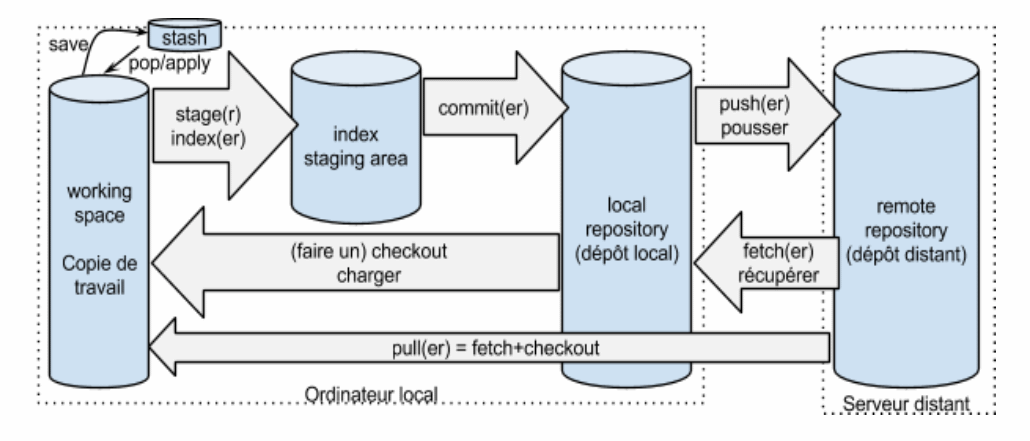
\includegraphics[scale=0.6]{images/technique_git.png}
\caption{Principe de fonctionnement d'un gestionnaire de versions}
\label{fonction}
\end{figure}

\section{Aperçu des gestionnaires de versions existants}

% idée : quels sont les différents gestionnaires de versions ? Qu'est-ce qui les différencie ? 
% & Comment sont-ils apparus ?
% - bitkeeper, git
% - cvs, svn

\subsection{CVS, centralisé}

CVS est l'un des plus anciens gestionnaires de versions. De ce fait, il n'est plus trop mis souvent à jour. Il est le moins puissant. 

\subsection{SVN, centralisé}

Avec GIT, il s'agit du gestionnaire de versions le plus utilisé. Il est simple d'utilisation et présente une interface graphique. 

\subsection{Mercurial, décentralisé}

Créé en même temps que GIT. 

\subsection{Bazaar, décentralisé}

Sur le même concept, il s'agit d'un outil conçu pour le projet Ubuntu et MySQL. 

\subsection{GIT, décentralisé}

Le meilleur, pour la fin, GIT est un outil récent, complet et puissant. Il est d'exécution rapide comparé à ses concurrents. Il est utilisé pour de multiples projets à ce jour. 

\subsection{Gestionnaires propriétaires}

Il existe des gestionnaires propriétaires, que nous nous contenterons de citer, car hors du cadre du logiciel libre. 
\begin{itemize}
\item BitKeeper
\item Perforce
\item Microsoft Visual SourceSafe
\end{itemize}

\section{Utilisation de GIT}
Cette partie a été réalisée à l'aide du livre Pro Git \cite{ProGit}. 

%@book{ProGit,
%author = {Scott Chacon},
%title = {Pro Git},
%date = {2008},
%}
%@ OPTurl = {http://git-scm.com/book/fr}, 
\subsection{Utilité}
\label{sec:utilite}

\par Pour un projet logiciel, la coopération de plusieurs personnes sur des fichiers communs est nécessaire, l'utilisation d'un gestionnaire de version s'impose. 
\par Il s'agit de pouvoir gérer les interventions simultanées de plusieurs opérateurs sur un même fichier et d'enregistrer progressivement les modifications apportées, tout en pouvant revenir dessus si nécessaire. Ce type de système est massivement utilisé aujourd'hui, pour les projets conséquents, ou impliquant la coopération de plusieurs personnes.
\par Github.com met à disposition une plateforme permettant d'héberger facilement des projets versionnés avec Git, c'est ce site que nous utiliserons.

\par Nous allons détailler les opérations à utiliser pour l'utilisation de Git en ligne de commande. 

\subsection{Création d'un projet}
\label{sec:creation-dun-projet}

\par Nous pouvons créer le projet avec les fonctionnalités intégrées de Github, mais en général, pour initialiser un projet git, on se place dans le répertoire du projet, à sa racine, puis on tape dans le terminal :
\begin{verbatim}
> git init
\end{verbatim}

\par Dans le cas d'un projet existant, on note l'adresse à laquelle le projet est disponible, par exemple \texttt{https://github.com/hhalex/PLS14}, et on tape dans le terminal:
\begin{verbatim}
> git clone https://github.com/hhalex/PLS14
\end{verbatim}

\par On verra normalement apparaître un dossier \texttt{.git} auquel il ne faudra surtout pas toucher puisqu'il s'agit des versions enregistrées par Git.

\subsection{Enregistrement des modifications}
\label{sec:enreg-des-modif}

\par En travaillant sur le projet, on peut enregistrer régulièrement les modifications localement. On effectue ainsi des points de sauvegarde, qu'on peut nommer explicitement afin de pouvoir s'y retrouver plus tard.
\par Après avoir apporté quelques modifications, placez-vous dans le répertoire du projet, à la racine, puis tapez :
\begin{verbatim}
> git status
\end{verbatim}
\par Cette commande va afficher tout d'abord les fichiers nouveaux/modifiés qui sont sélectionnés pour l'enregistrement, puis les fichiers nouveaux/modifiés non sélectionnés. 

\begin{verbatim}
Alex > 
# On branch master
# Changes not staged for commit:
#   (use "git add <file>..." to update what will be committed)
#   (use "git checkout -- <file>..." to discard changes in working directory)
#
#	modified:   CompteRendu/page_garde.tex
#	modified:   CompteRendu/partie1.tex
#	modified:   CompteRendu/partie2.tex
#
# Untracked files:
#   (use "git add <file>..." to include in what will be committed)
#
#	CompteRendu/.#partie2.tex
#	CompteRendu/CompteRendu.aux
#	CompteRendu/CompteRendu.idx
#	CompteRendu/CompteRendu.log
#	CompteRendu/CompteRendu.pdf
#	CompteRendu/CompteRendu.synctex.gz
#	CompteRendu/CompteRendu.toc
#	CompteRendu/auto/
#	CompteRendu/page_garde.aux
#	CompteRendu/partie1.aux
#	CompteRendu/partie2.aux
#	CompteRendu/partie3.aux
#	CompteRendu/partie4.aux
#	CompteRendu/partie5.aux
#	CompteRendu/styles.aux
no changes added to commit (use "git add" and/or "git commit -a")
\end{verbatim}

\par Dans l'exemple précédent, aucun fichier n'est sélectionné pour le prochain enregistrement, appelé \emph{commit} dans le jargon de Git. On voit néanmoins apparaître 3 fichiers modifiés : \texttt{page\_garde.tex}, \texttt{partie1.tex}, \texttt{partie2.tex} encore non ajoutés à la liste des fichiers pour le prochain commit. Toute une série de fichiers divers apparaissent comme \emph{untracked}, dans notre cas il ne s'agit que de fichiers temporaires utiles pour la compilation du présent document. 

\par Pour sélectionner les fichiers à ajouter au prochain enregistrement, tapez :
\begin{verbatim}
> git add fichier 
\end{verbatim}

\par On peut aller plus vite en donnant le nom du \texttt{dossier} pour ajouter tous les fichiers contenus dans \texttt{dossier}. Par exemple, si on avait voulu enregistrer tous les fichiers temporaires générés par la compilation du compte rendu, on aurait pu taper :
\begin{verbatim}
> git add CompteRendu
\end{verbatim}

\par Maintenant que les fichiers intéressants ont été sélectionnés, on peut procéder à l'étape d'enregistrement. Toujours au même endroit dans le dossier du projet, tapez :
\begin{verbatim}
> git commit -m "description du commit"
\end{verbatim}

\par Par exemple :
\begin{verbatim}
 > git commit -m "[CompteRendu] Modification de la page de garde"
[master afe15b1] [CompteRendu] Modification de la page de garde
 1 file changed, 10 insertions(+), 5 deletions(-)
\end{verbatim}

\par Vous pouvez maintenant vérifier que votre commit est bien là en tapant :
\begin{verbatim}
> git log
\end{verbatim}

\par Dans notre exemple :

\begin{verbatim}
> git log
commit afe15b1adda058c10e066d0c01b40ec950eb2911
Author: alexandre <alexandre.careil@supelec.fr>
Date:   Sun Feb 16 16:31:51 2014 +0100

    [CompteRendu] Modification de la page de garde

commit 4f1aa9118121e69652afc65548b2efc2445ff699
Author: alexandre <alexandre.careil@supelec.fr>
Date:   Sun Feb 16 16:31:24 2014 +0100

    [git] modification du .gitignore

commit 0f548ee172c523eaaa6c51e9db113096470fba3f
Author: ThiDiff <juanmanuel.munozperez@gmail.com>
Date:   Thu Feb 13 10:18:38 2014 +0100

    [GUI] Ajout de la classe Fenetre
\end{verbatim}


\par Cette commande affiche la liste des commits effectués sur le projet. Vous pouvez vous apercevoir que certains commits ne sont pas de vous.

\subsection{Synchronisation avec le projet de référence}
\label{sec:synchr-avec-le}

\par Une fois toutes vos modifications effectuées et bien enregistrées comme indiqué dans le paragraphe précédent, il faut les rendre accessibles à toutes les autres personnes qui travaillent également sur le projet. Il faut d'abord commencer par récupérer les éventuelles modifications qui auraient pu être ajoutées pendant votre travail. Pour cela on crée une branche \texttt{pull} sur laquelle on récupère le projet distant, puis on le fusionne avec votre version.

\par On crée la branche \texttt{pull}
\begin{verbatim}
> git checkout -b pull
\end{verbatim}

\par On récupère la dernière version du projet :
\begin{verbatim}
> git pull adresse_du_projet master
\end{verbatim}

\par Dans notre cas :
\begin{verbatim}
> git pull https://github.com/hhalex/PLS14 master
\end{verbatim}

\par Une fois fait, on retourne sur la branche \texttt{master} (la branche de base) et on fusionne le contenu de \texttt{pull} :

\begin{verbatim}
> git checkout master
> git merge pull
\end{verbatim}

\par Dans notre exemple :

\begin{verbatim}
Alex > git pull https://github.com/hhalex/PLS14 master
From https://github.com/hhalex/PLS14
 * branch            master     -> FETCH_HEAD
Already up-to-date.
Alex > git checkout master
Switched to branch 'master'
Your branch is ahead of 'origin/master' by 2 commits.
  (use "git push" to publish your local commits)
Alex > git merge pull
Already up-to-date.
\end{verbatim}

\par Maintenant que votre branche \texttt{master} est fin prête, on peut l'envoyer sur le projet distant. Pour cela, tapez :

\begin{verbatim}
> git push https://github.com/hhalex/PLS14 master
\end{verbatim}

\par Dans notre exemple :
\begin{verbatim}
 > git push https://github.com/hhalex/PLS14 master
Username for 'https://github.com': hhalex
Password for 'https://hhalex@github.com': ****

Counting objects: 10, done.
Delta compression using up to 4 threads.
Compressing objects: 100% (7/7), done.
Writing objects: 100% (7/7), 975 bytes | 0 bytes/s, done.
Total 7 (delta 4), reused 0 (delta 0)
To https://github.com/hhalex/PLS14
   0f548ee..afe15b1  master -> master
\end{verbatim}

\subsection{Nettoyage des branches}
\label{sec:nett-des-branch}

\par Maintenant que l'étape de synchronisation est effectuée, la branche \texttt{pull} n'est plus nécessaire, vous pouvez donc la supprimer :
\begin{verbatim}
> git branch -d pull
\end{verbatim}

\section*{Conclusion}

Cette étude nous a permis d'explorer l'origine des gestionnaires de versions ainsi que de comprendre les différences entre les solutions proposées. Elle nous a conforté dans le choix de GIT, qui est un outil décentralisé, robuste et flexible. 


%%% Local Variables: 
%%% mode: latex
%%% TeX-master: "rapport_master"
%%% End: 
